\begin{frame}
  \maketitle
\end{frame}

\begin{frame}
  \frametitle{Piano della presentazione}
  \tableofcontents
\end{frame}

\section{Introduzione}

\begin{frame}
  \frametitle{Cos'è?}
  \begin{block}{Energia oscura}
    Forma di energia che permea l'Universo.
  \end{block}
  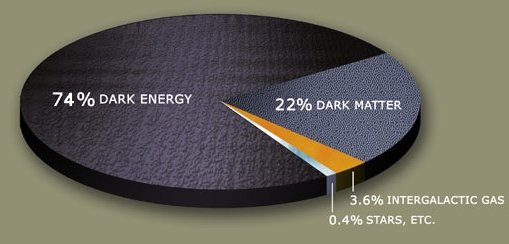
\includegraphics[width=\columnwidth]{DarkMatterPie}
\end{frame}

\section[Origine]{Origine dell'energia oscura}

\begin{frame}
  \frametitle{Perché serve l'energia oscura?}
  L'Universo si sta espandendo in maniera \alert{accelerata}.
  \begin{figure}
    \centering
    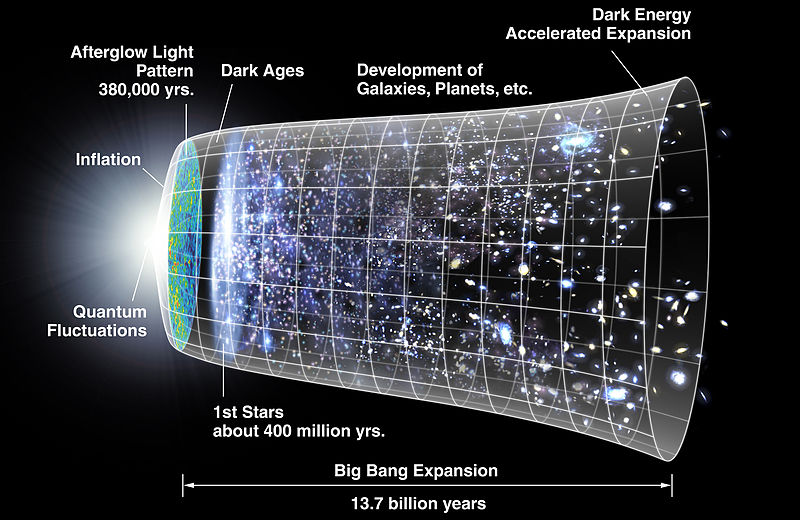
\includegraphics[width=0.9\columnwidth]{800px-CMB_Timeline300_no_WMAP}
  \end{figure}
\end{frame}

\begin{frame}
  \frametitle{Prove dell'espansione accelerata dell'Universo}
  \begin{itemize}[<+->]
  \item Supernove di tipo Ia (Riess e Perlmutter, 1998)
  \item Radiazione cosmica di fondo
  \item Struttura a grande scala dell'Universo
  \end{itemize}
\end{frame}

\section[Natura]{Natura dell'energia oscura}

\begin{frame}
  \frametitle{Cos'è precisamente l'energia oscura?}
  Ci sono varie ipotesi
  \begin{itemize}
  \item Costante cosmologica
  \item Quintessenza
  \item Altre idee alternative
  \end{itemize}
\end{frame}

\begin{frame}
  \frametitle{Che caratteristiche ha?}
  Indipendentemente dalle ipotesi sulla natura l'energia oscura deve avere
  \alert{pressione negativa}. Serve per giustificare l'accelerazione
  nell'espansione.
\end{frame}

\begin{frame}
  \frametitle{Costante cosmologica}
  Densità costante ed estremamente bassa blablabla...
\end{frame}

\begin{frame}
  \frametitle{Quintessenza}
  Densità variabile in spazio e tempo blablabla...
\end{frame}

\section[Conseguenze]{Conseguenze nel destino dell'Universo}

\begin{frame}
  \frametitle{Quale sarà la fine dell'Universo?}
  Dipende fortemente dalla reale densità di energia e materia oscure.
  \begin{figure}
    \centering
    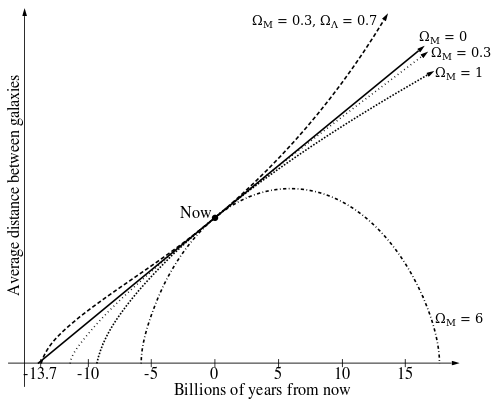
\includegraphics[width=0.7\columnwidth]{500px-Friedmann_universes}
  \end{figure}
\end{frame}

%%% Local Variables: 
%%% mode: latex
%%% TeX-master: "seminario"
%%% End: 
